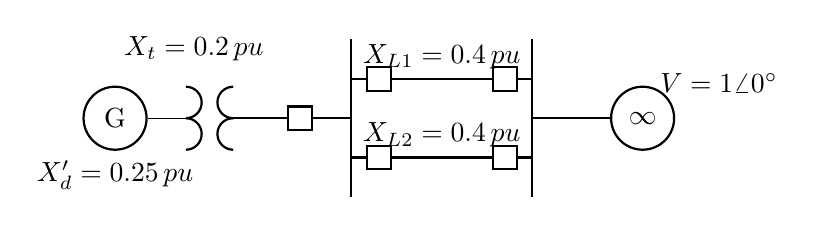
\begin{tikzpicture}
    % Generator
    \node[circle, draw, thick, minimum size=0.8cm, inner sep=0] (G) at (0,0) {G};
    \node[below] at (G.south) {$X_d' = 0.25 \, \text{pu}$};

    % Transformer reactance Xt
    \draw (G.east) -- ++(0.5, 0);
    \draw[thick] (1.5,0.4) arc[start angle=90,end angle=270,radius=0.2cm];
    \draw[thick] (1.5,-0) arc[start angle=90,end angle=270,radius=0.2cm];
    \draw[thick] (0.9,0) arc[start angle=270,end angle=450,radius=0.2cm];
    \draw[thick] (0.9,-.4) arc[start angle=270,end angle=450,radius=0.2cm];
    \node[above] at (1,0.6) {$X_t = 0.2 \, \text{pu}$};

    % Transmission line
    \draw[thick] (1.5,0) -- (2.2,0);
    \draw[thick] (2.2, -0.15) rectangle (2.5, 0.15);
    \draw[thick] (2.5, 0) -- (3, 0);
    \draw[thick] (3,-1) -- (3,1);  % Bus line

    % Inductors X_L1 and X_L2
    % Upper inductor X_L1
    \draw[thick] (3,0.5) -- (3.2, 0.5);
    \draw[thick] (3.2, 0.35) rectangle (3.5, 0.65);
    \draw[thick] (3.5,0.5) -- (4.8,0.5) node[midway, above] {$X_{L1} = 0.4 \, \text{pu}$};
    \draw[thick] (4.8,0.35) rectangle (5.1,0.65);
    \draw[thick] (5.1,0.5) -- (5.3,0.5);
    
    % Lower inductor X_L2
    \draw[thick] (3,-0.5) -- (3.2, -0.5);
    \draw[thick] (3.2, -0.35) rectangle (3.5, -0.65);
    \draw[thick] (3.5,-0.5) -- (4.8,-0.5) node[midway, above] {$X_{L2} = 0.4 \, \text{pu}$};
    \draw[thick] (4.8,-0.35) rectangle (5.1,-0.65);
    \draw[thick] (5.1,-0.5) -- (5.3,-0.5);

    % Right side bus line
    \draw[thick] (5.3,-1) -- (5.3,1);
    
    % Infinite bus
    \draw[thick] (5.3,0) -- ++(1,0);
    \node[circle, draw, thick, minimum size=0.8cm, inner sep=0] (inf) at (6.7,0) {};
    \node at (inf) {\(\infty\)};
    \node[above right] at (6.8,0.2) {$V = 1 \angle 0^\circ$};
\end{tikzpicture}
